% ============================================
% 第3章 系统需求分析
% ============================================
\section{系统需求分析}

本章详细分析了基于 Next.js 的在线问卷系统的需求，明确系统的核心功能。
根据使用对象的不同，通过使用用例图的方式对系统需求进行进一步的分析，
最终完成对系统的需求分析。

\subsection{需求概述}

\subsubsection{业务需求概述}

随着互联网技术的快速发展，在线问卷调查已成为数据收集的重要手段，
广泛应用于市场调研、学术研究、用户反馈、满意度评估等诸多场景。
当前，国内外已涌现出众多在线问卷平台，如国外的 SurveyMonkey、Google Forms，
国内的问卷星、腾讯问卷等。这些平台功能成熟、用户基数庞大，
但在实际使用中也暴露出一些共性问题：一是协作能力薄弱，
多人共同编辑问卷时缺乏实时同步机制；二是智能化程度不足，
问卷设计和数据分析仍高度依赖人工经验；三是版本管理缺失，
问卷内容频繁修改时缺乏有效的版本回溯机制。

在此背景下，本系统旨在为个人用户和中小团队提供一个功能完善、
支持实时协作、具备 AI 智能辅助的在线问卷平台。
系统的业务需求主要集中在以下方面：

\begin{enumerate}[label=(\arabic*)]
  \item 提供可视化问卷编辑器，支持丰富的题型（18种）与灵活的问卷设计；
  \item 实现问卷发布与版本快照管理，保障已收集数据与题目结构的一致性；
  \item 集成 DeepSeek 大语言模型，实现问卷智能生成与数据分析总结；
  \item 支持多人实时协作编辑，通过题目级乐观锁定避免编辑冲突；
  \item 提供多维度的数据统计与可视化展示，帮助用户从数据中获取洞察。
\end{enumerate}

\subsubsection{目标用户}

基于在线问卷系统的实际应用场景，依据业务需求划分成三类角色：
\textbf{问卷创建者}、\textbf{问卷填写者}、\textbf{协作者}。
各角色用户的具体功能描述如下：

\textbf{(1) 问卷创建者}

系统的核心用户，拥有问卷的所有权。可以进行问卷的创建、编辑、发布、
版本管理、结果统计等全部操作。问卷创建者可邀请其他用户作为协作者
共同编辑问卷，并设置协作者的权限（仅查看/可编辑/可查看结果）。

\textbf{(2) 问卷填写者}

通过公开链接访问并填写问卷的匿名用户或注册用户。无需登录即可
访问已发布的问卷，完成答题后提交答案。系统会自动采集答题者的
设备信息和地理位置，用于后续统计分析。

\textbf{(3) 协作者}

受问卷创建者邀请参与协作的用户。根据被授予的权限，协作者可以
在编辑器中实时查看和修改问卷内容，或查看问卷的统计结果。
协作者通过邀请码或邀请链接加入协作。

\subsection{功能需求分析}

\subsubsection{问卷创建者需求分析}

问卷创建者是系统的主要使用者，其核心需求是完整地管理问卷从创建到
数据分析的整个生命周期。如图~\ref{fig:use-case-creator} 所示，
问卷创建者的功能需求包括：

\begin{itemize}
  \item \textbf{用户认证}：支持邮箱密码注册登录、Google OAuth、GitHub OAuth 三种认证方式；
  \item \textbf{问卷管理}：创建、查看、编辑、删除问卷，问卷列表展示基本信息（标题、题目数、回答数、发布状态）；
  \item \textbf{问卷编辑}：使用可视化编辑器设计问卷，支持 18 种题型（单选、多选、矩阵、评分、NPS 等），支持拖拽排序、实时预览；
  \item \textbf{问卷发布}：发布问卷生成唯一分享链接（\texttt{shareToken}），支持取消发布；
  \item \textbf{版本管理}：创建版本快照、查看历史版本列表、回滚到指定版本、删除历史版本；
  \item \textbf{结果统计}：查看数据概览（回收量、完成率、趋势图）、逐题统计图表、数据详情表格（搜索、筛选、分页、CSV 导出）、交叉分析、AI 智能总结；
  \item \textbf{协作管理}：生成邀请码/邀请链接，邀请用户加入协作，管理协作者权限（查看/编辑/查看结果）；
  \item \textbf{AI 辅助}：通过自然语言描述需求，由 AI 自动生成问卷题目；基于回收数据生成智能分析总结报告。
\end{itemize}

\begin{figure}[H]
\centering
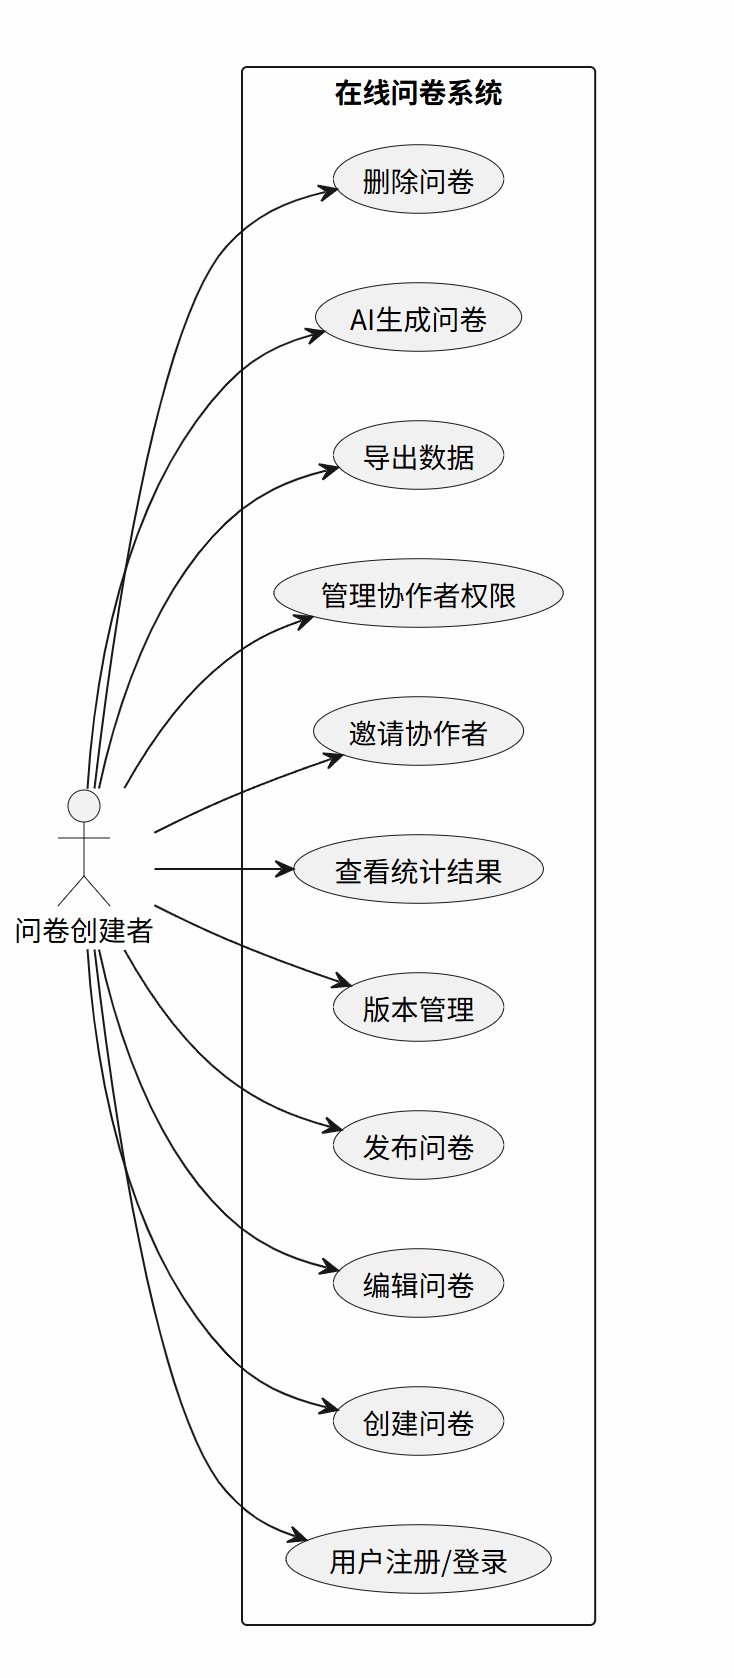
\includegraphics[width=0.55\textwidth]{figures/use-case-creator.png}
\caption{问卷创建者用例图}
\label{fig:use-case-creator}
\end{figure}

\subsubsection{问卷填写者需求分析}

问卷填写者通过公开链接访问问卷，其核心需求是流畅地完成答题并提交。
如图~\ref{fig:use-case-respondent} 所示，具体功能需求包括：

\begin{itemize}
  \item \textbf{访问问卷}：通过 \texttt{/s/\{shareToken\}} 链接访问已发布的问卷；
  \item \textbf{浏览题目}：查看问卷标题、描述及各题目内容；
  \item \textbf{填写答案}：根据题型要求选择或输入答案，系统提供前端必填校验；
  \item \textbf{提交问卷}：完成答题后提交，系统返回提交成功确认。
\end{itemize}

\begin{figure}[H]
\centering
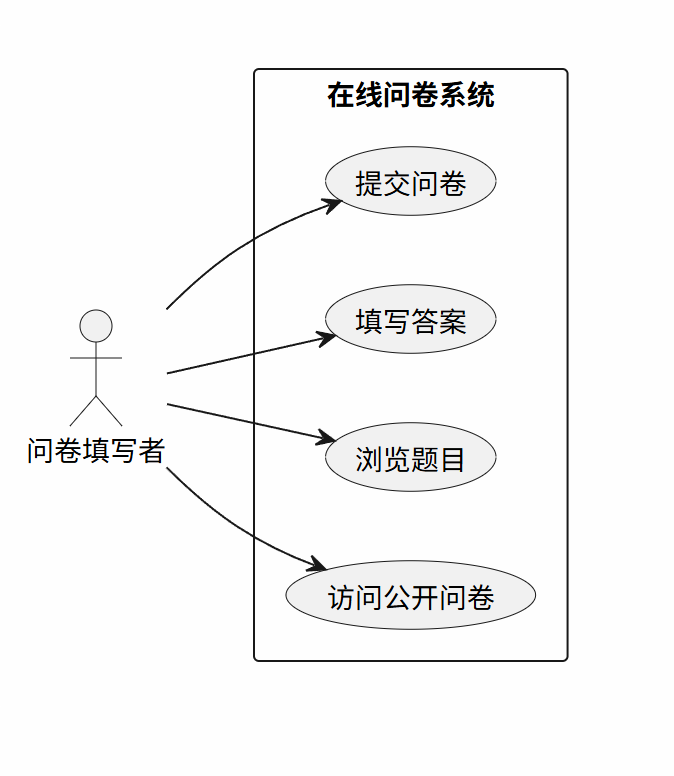
\includegraphics[width=0.75\textwidth]{figures/use-case-respondent.png}
\caption{问卷填写者用例图}
\label{fig:use-case-respondent}
\end{figure}

\subsubsection{协作者需求分析}

协作者受创建者邀请参与问卷协作，根据被授予的权限分为"可编辑"和
"可查看结果"两类。如图~\ref{fig:use-case-collaborator} 所示，
其功能需求包括：

\begin{itemize}
  \item \textbf{加入协作}：通过邀请码或邀请链接加入问卷协作，确认加入后获得相应权限；
  \item \textbf{编辑问卷}：在编辑器中查看和修改问卷内容（需具备编辑权限）；
  \item \textbf{实时协作}：参与多人实时协作编辑，系统通过题目级乐观锁定避免冲突，实时同步题目增删改、重排等变更；
  \item \textbf{查看结果}：查看问卷统计数据和可视化图表（需具备查看结果权限）。
\end{itemize}

\begin{figure}[H]
\centering
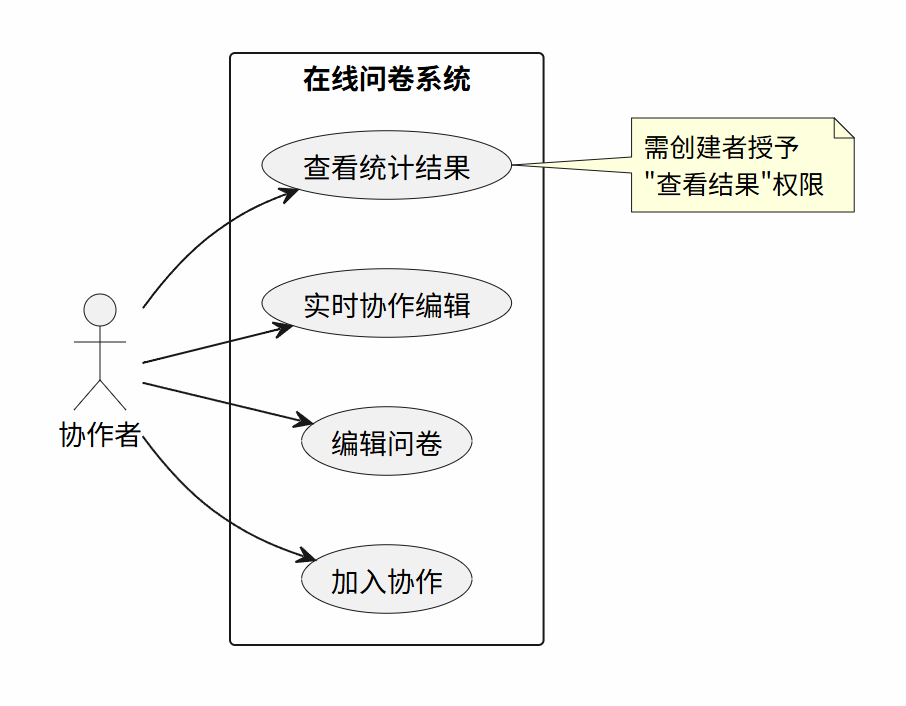
\includegraphics[width=0.55\textwidth]{figures/use-case-collaborator.png}
\caption{协作者用例图}
\label{fig:use-case-collaborator}
\end{figure}

\subsection{非功能需求分析}

除上述功能需求外，系统还需满足以下非功能需求，以保障系统的稳定性、
安全性和用户体验：

\begin{table}[H]
\centering
\caption{系统非功能需求}
\label{tab:non-functional-requirements}
\begin{tabular}{lp{10cm}}
\toprule
\textbf{需求类型} & \textbf{具体要求} \\
\midrule
性能 & 页面首屏加载时间 $<$ 3s，API 响应时间 $<$ 500ms，
编辑器首屏加载时间 $<$ 2.5s \\
可用性 & 系统可用性 $>$ 99\%，支持并发用户访问，
Pusher 实时协作延迟 $<$ 200ms \\
安全性 & 用户密码 bcrypt 加密存储（cost=12），
API JWT 鉴权，SQL 注入防护，HTTPS 传输 \\
可扩展性 & 模块化架构，题型注册中心模式支持新题型即插即用，
功能模块松耦合 \\
兼容性 & 支持主流桌面浏览器（Chrome、Firefox、Safari、Edge），
问卷填写页适配移动端 \\
\bottomrule
\end{tabular}
\end{table}

\subsection{本章小结}

本章对基于 Next.js 的在线问卷系统的需求进行了详细的分析。
首先明确了系统的业务背景与核心目标，指出现有平台在协作、
智能化和版本管理方面的不足。随后依据业务场景划分了三类目标用户：
问卷创建者、问卷填写者和协作者，并分别从各角色的视角出发，
详细分析了其功能需求，绘制了对应的用例图。
最后列出了系统的非功能需求，涵盖性能、可用性、安全性、
可扩展性和兼容性五个维度。

本章的需求分析为后续的系统架构设计、数据库设计和核心模块实现
奠定了基础，确保系统开发能够紧密围绕用户实际需求展开。
